%%%%%%%%%%%%%%%%%%%%%%%%%%%%%%%%%%%%%%%%%%%%%%%%%%%%%%%%%%%%
% Document settings
\documentclass{ACGSeminar}

\bibliography{references}

%%%%%%%%%%%%%%%%%%%%%%%%%%%%%
% Hyphenations here
%%%%%%%%%%%%%%%%%%%%%%%%%%%%%
\hyphenation{}

%%%%%%%%%%%%%%%%%%%%%%%%%%%%%
% Title, Author, etc.

\begin{document}

\title{Being the Perfect Employee at the Crusty Crab 123}

\author{Spongebob Squarepants}

\maketitle

%%%%%%%%%%%%%%%%%%%%%%%%%%%%%%%%%%%%%%%%%%%%%%%%%%%%%%%%%%%%
% Abstract

\begin{abstract}%
Lorem ipsum dolor sit amet, consetetur sadipscing elitr, sed diam nonumy eirmod
tempor invidunt ut labore et dolore magna aliquyam erat, sed diam voluptua. At
vero eos et accusam et justo duo dolores et ea rebum. Stet clita kasd
gubergren, no sea takimata sanctus est Lorem ipsum dolor sit amet. Lorem ipsum
dolor sit amet, consetetur sadipscing elitr, sed diam nonumy eirmod tempor
invidunt ut labore et dolore magna aliquyam erat, sed diam voluptua. At vero
eos et accusam et justo duo dolores et ea rebum. Stet clita kasd gubergren, no
sea takimata sanctus est Lorem ipsum dolor sit amet.
\end{abstract}

\keywords{My first keyword, my second keyword}
\tableofcontents

%%%%%%%%%%%%%%%%%%%%%%%%%%%%%%%%%%%%%%%%%%%%%%%%%%%%%%%%%%%%
% Introduction

\section{Introduction}

Introduction to your exciting topic including
some citation~\cite{Plankton2003}. Define citations
in \verb+references.bib+ that you find in
the latex source folder.

%%%%%%%%%%%%%%%%%%%%%%%%%%%%%%%%%%%%%%%%%%%%%%%%%%%%%%%%%%%%
% Second Section

\section{My Fancy Second Section}

My second section is even better than the
first one\footnote{Proof omitted.}
because it contains a footnote as well as another
citation~\cite{Plankton2011}. Everything else is
explained in Figure~\ref{fig:dummy}. Always make sure
that all figures are referenced.

\begin{figure}[htb!]
  \begin{centering}
    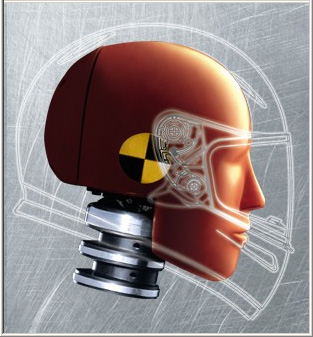
\includegraphics[width=4cm]{figures/dummy.jpg}\par
  \end{centering}
  \caption{A simple dummy picture to demonstrate how
           to include graphics into your report.}
  \label{fig:dummy}
\end{figure}

%%%%%%%%%%%%%%%%%%%%%%%%%%%%%%%%%%%%%%%%%%%%%%%%%%%%%%%%%%%%
% Bibliography

\printbibliography
\cleardoublepage

\end{document}
